\documentclass[14pt]{article}
\usepackage[14pt]{extsizes}
\usepackage[utf8]{inputenc}
\usepackage[T2B]{fontenc}
\usepackage[english,russian]{babel}
\usepackage{amsmath}
\usepackage{amssymb}
\usepackage{hyperref}
\usepackage{longtable}
\usepackage[table]{xcolor}  
\usepackage{array}
\usepackage{color}
\usepackage{xcolor}
\usepackage{hyperref}
\usepackage{listings}
\usepackage{alltt}
\usepackage{csquotes}
\usepackage{graphicx}
\usepackage{listings}
\usepackage{longtable}
\usepackage{fullpage}
\usepackage{multicol,multirow}
\usepackage{tabularx}
\usepackage{ulem}

\lstset{tabsize=2,
	breaklines,
	columns=fullflexible,
	flexiblecolumns,
	numbers=left,
	numberstyle={\footnotesize},
	extendedchars =\true}

\begin{document}

\begin{titlepage}
\begin{center}
\bfseries

{\Large Московский авиационный институт\\ (национальный исследовательский университет)}

\vspace{48pt}

{\large Факультет информационных технологий и прикладной математики}

\vspace{24pt}

{\large Кафедра вычислительной математики и~программирования}

\vspace{48pt}

{\largeКурсовой проект по курсу \enquote{Дискретный анализ}}
\vspace{24pt}

{\large Разработка архиватора (Huffman + LZ77)}

\end{center}

\vspace{72pt}

\begin{flushright}
\begin{tabular}{rl}
Студент: & Фирфаров А.С. \\
Преподаватель: & Журавлев А.А. \\
Группа: & М8О-208Б \\
Дата: & \\
Оценка: & \\
Подпись: & \\
\end{tabular}
\end{flushright}

\vfill

\begin{center}
\bfseries
Москва, 2019
\end{center}
\end{titlepage}
\pagebreak

\section*{Курсовой проект}

Необходимо спроектировать и реализовать архиватор, использующий заданные  методы сжатия данных для сжатия одного файла. \\

\noindentФормат запуска должен быть аналогичен формату запуска программы gzip, должны быть поддержаны следующие ключи:  \mbox{-c, -d, -k, -l, -r, -t, -1, -9}. Должно поддерживаться указание символа дефиса в качестве стандартного ввода.

\pagebreak

\section*{Теоретическая часть}

LZ77 -  алгоритм сжатия без потерь, опубликованный в статье израильских математиков Авраама Лемпеля и Яакова Зива в 1977 году. Многие программы сжатия информации используют ту или иную модификацию этого алгоритма. LZ77 относится к словарным алгоритмам сжатия, в котором словарь формируется на основании уже обработанной части входного потока. Алгоритм использует скользящее окно, разделенное на две неравные части. Первая, большая по размеру, включает уже просмотренную часть сообщения. Вторая, намного меньшая, является буфером, содержащим еще незакодированные символы входного потока. Идея алгоритма заключается в поиске самого длинного совпадения между строкой буфера и всеми фразами словаря. Полученная в результате поиска фраза кодируется с помощью двух чисел и одного символа: смещения от начала буфера(offset), длины совпадения(length) и символа, следующего за совпавшей строкой буфера. Затем окно смещается на length + 1 символ вправо и алгоритм повторяется. Алгоритм имеет следующие недостатки: невозможность кодирования подстрок, стоящих друг от друга на расстоянии, большем длины словаря, малая эффективность при кодировании незначительных объёмов данных и ограничнность длины подстроки, которую можно закодировать. \\

\noindentАлгоритм Хаффмана — жадный алгоритм оптимального префиксного кодирования. Алгоритм был разработан в 1952 году аспирантом Массачусетского технологического института Дэвидом Хаффманом. Идея алгоритма заключается в замене символов на соответствующие им коды. Часто встречающимся символам будут соответствовать меньшие коды, редко встречающиеся символы получат более длинные коды. Это нужно для того, чтобы самые частотные символы занимали как можно меньше места. Ни один из кодов не является префиксом другого, что позволяет их однозначно интерпретировать. Алгоритм хорошо дополняет LZ77, позволяя улучшить степень сжатия.
\pagebreak

\section*{Реализация}
На первом этапе текст сжимается с помощью алгоритма LZ77. Ищется совпадение между словарем и буфером, и найденное самое длинное совпадение записывается во временный файл в виде упорядоченной тройки <смещение(offset), длина совпадения(length), следующий символ(nextChar)>. На каждой итерации алгоритма совпадение между словарем и буфером ищется с помощью  \mbox{Z-функции.} Формируется вспомогательная строка вида "буфер" + "символ разделитель" + "словарь" + "буфер". Z - функция для этой строки вычисляется за линейное время. Таким образом можно найти длину наибольшего совпадения и его позицию в словаре. По мере записи закодированных последовательностей во временных файл, собирается статистика "символов"\  для полустатического алгоритма Хаффмана. Это позволит не делать лишний проход по сжатому алгоритмом LZ77 тексту. Степень сжатия зависит от максимального размера словаря. Большой словарь позволяет найти большее совпадение, но за значительное время. Меньший словарь позволяет тратить меньше времени на поиск совпадений,  но качество сжатия будет хуже. 

\begin{figure}[h]
\centering
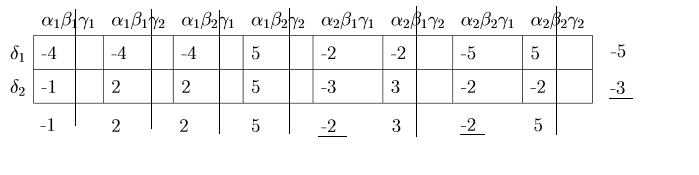
\includegraphics[width=1\linewidth]{11.png}
\caption{Зависимость времени сжатия от размера словаря - файл 80 MB}
\label{fig:mpr}
\end{figure}

\pagebreak

\begin{figure}[h]
\centering
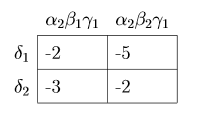
\includegraphics[width=1\linewidth]{12.png}
\caption{Зависимость степени сжатия (\%) от размера словаря - файл 80 MB}
\label{fig:mpr}
\end{figure}

\noindentДалее полученный временный файл сжимается полустатическим алгоритмом Хаффмана. Статистика частот для каждого байта была собрана на предыдущем шаге, поэтому нет необходимости просматривать временный файл для этого. На основании этой статистики строится дерево кодов Хаффмана. При построении используется очередь с приоритетами.  Время, затраченное на построение дерева, несущественно по сравнению с временем дальнейшего кодирования. Для разархивации необходимо записать в конечный файл сереализованное дерево кодов Хаффмана. Далее каждый байт заменяется на соответствующий ему код и записывается в выходной файл. \\

\noindentДля разархивации дерево кодов Хаффмана нужно десереализовать и заменить коды из архива на соответствующие им байты. Далее к полученному временному файлу применяется алгоритм декодирования LZ77. В результате получается исходный несжатый файл.

\pagebreak

\section*{Сравнение с аналогами}

\begin{figure}[h]
\centering
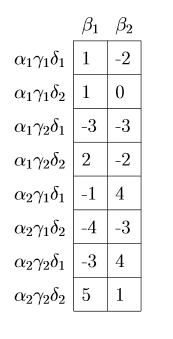
\includegraphics[width=1\linewidth]{21.png}
\caption{Сравнение степени сжатия}
\label{fig:mpr}
\end{figure}

\noindentВидно, что архиватор проигрывает по степени сжатия архиватору gzip. Можно добиться схожей степени сжатия, существенно увеличив размер буфера и словаря, но это также сильно увеличит время сжатия. Стоит отметить, что при сжатии маленьких файлов размер архива может быть даже больше размера оригинального файла. Это связано с необходимостью хранить дерево кодов Хаффмана и другую дополнительную информацию.

\pagebreak

\begin{figure}[h]
\centering
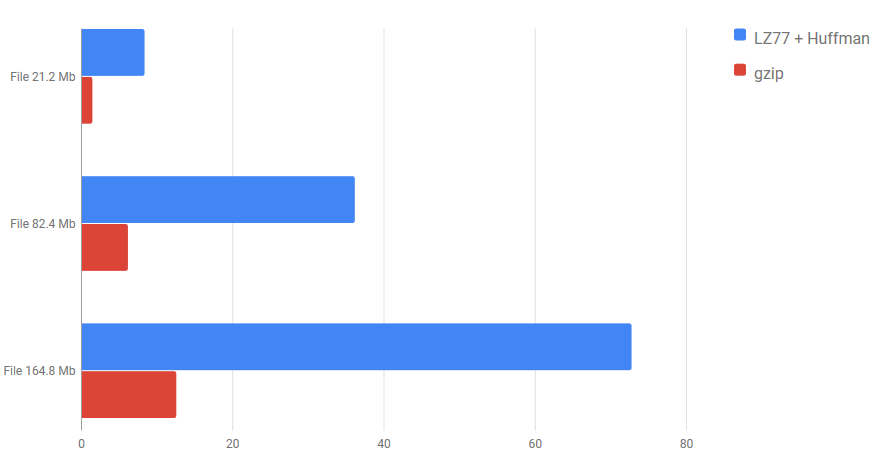
\includegraphics[width=1\linewidth]{22.png}
\caption{Сравнение времени сжатия}
\label{fig:mpr}
\end{figure}

\pagebreak

\section*{Исходный код}

\begin{lstlisting}[language=C++]
#include <iostream>
#include <fstream>
#include <string>
#include <vector>
#include <queue>
#include <memory>
#include <unordered_map>
#include <experimental/filesystem>

#define TEST_NUMBER 1234567890
#define MAX_DICT_SIZE 255
#define MIN_DICT_SIZE 80

uint8_t DICT_SIZE = 168;
const uint8_t AHEAD_SIZE = 8;
const uint8_t BYTE_SIZE = 8;

struct LZ77Code {
    uint8_t offset;
    uint8_t length;
    char nextChar;
};

struct HuffTreeNode {
    HuffTreeNode() {};
    HuffTreeNode(const std::shared_ptr<HuffTreeNode>& _left, const std::shared_ptr<HuffTreeNode>& _right) {
        left = _left;
        right = _right;
        freq = left->freq + right->freq;
    }
    HuffTreeNode(int _freq, char _symb) : freq(_freq), symb(_symb), leaf(true) {};

    bool leaf = false; 
    char symb;
    int freq;

    std::shared_ptr<HuffTreeNode> left = nullptr;
    std::shared_ptr<HuffTreeNode> right = nullptr;
};

struct CompareNodes {
    bool operator()(const std::shared_ptr<HuffTreeNode>& node1, const std::shared_ptr<HuffTreeNode>& node2) {
        return node1->freq > node2->freq;
    }
};

LZ77Code FindMatch(const std::string& data, int startDict, int startAhead, int endAhead) {
    
    std::string s1 = data.substr(startAhead, endAhead - startAhead + 1) + char(245);
    std::string s2 = data.substr(startDict, endAhead - startDict + 1);
    std::string text = s1 + s2;
    std::vector<int> z(text.size() - (endAhead - startAhead + 1), 0);

    int left = 0;
    int right = 0;

    uint8_t offset = 0;
    uint8_t length = 0;
    char next = data[startAhead];

    int size = z.size();
 
    for (int i = 1; i < size; ++i) {
        if (i <= right) {
            z[i] = std::min(right - i + 1, z[i - left]);
        }
        while (i + z[i] < size && text[z[i]] == text[i + z[i]]) {
            ++z[i];
        }

        if (i > endAhead - startAhead + 1 && z[i] > length) {
            length = z[i];
            offset = size - i;
            next = startAhead + length < data.size() ? data[startAhead + length] : '\0';
            if (length == endAhead - startAhead + 1) return {offset, length, next};
        }

        if (i + z[i] - 1 > right) {
            left = i;
            right = i + z[i] - 1;
        }
    }
    return {offset, length, next};
}

void LZ77Compress(const std::string& fileName, const std::string& data, std::unordered_map<char, int>& stat) {

    std::ofstream output(fileName + ".tmp", std::ios::binary);

    if (data.empty()) {
        LZ77Code last = {0, 0, '\0'};

        stat[0] += 2; 
        ++stat['\0'];

        output.write((char*)(&last), sizeof(LZ77Code));  

        output.close();
        return;
    }

    LZ77Code firstCode = {0, 0, data[0]};

    stat[0] += 2; 
    ++stat[data[0]];

    output.write((char*)(&firstCode), sizeof(LZ77Code));

    if (data.size() == 1) {
        LZ77Code last = {0, 0, '\0'};

        stat[0] += 2; 
        ++stat['\0'];

        output.write((char*)(&last), sizeof(LZ77Code));  
        output.close();
        return;
    }

    int startDict = 0;
    int startAhead = 1;
    int endAhead = data.size() - 1 > AHEAD_SIZE ? AHEAD_SIZE : data.size() - 1; 

    while (true) {
        LZ77Code code = FindMatch(data, startDict, startAhead, endAhead);
        
        ++stat[code.offset];
        ++stat[code.length]; 
        ++stat[code.nextChar];

        output.write((char*)(&code), sizeof(LZ77Code));
        if (code.nextChar == '\0') break;

        startAhead += code.length + 1;
        startDict = startAhead - DICT_SIZE >= 0 ? startAhead - DICT_SIZE : 0;
        endAhead = startAhead + AHEAD_SIZE < data.size() ? startAhead + AHEAD_SIZE - 1 : data.size() - 1;

        if (startAhead >= data.size()) {
            LZ77Code last = {0, 0, '\0'};

            stat[0] += 2; 
            ++stat['\0'];

            output.write((char*)(&last), sizeof(LZ77Code));            
            break;
        }
    }

    output.close();
    return;
}

void LZ77Decompress(const std::string& fileName) {

    std::ofstream output(fileName, std::ios::out);
    std::ifstream input(fileName + ".tmp", std::ios::binary | std::ios::in);
    std::string text;
    LZ77Code code;

    while(input) {

        input.read((char*)(&code), sizeof(LZ77Code));

        if (code.length > 0) {
            uint64_t start = text.length() - code.offset;
            for (int i = 0; i < code.length; ++i) {
                text += text[start + i];
            }
        }
        if (code.nextChar == '\0') break;
        text += code.nextChar;
    } 
    output << text;

    output.close();
    input.close();

    std::string removeFile = fileName + ".tmp";
    remove(removeFile.c_str());
}

void CreateCodesCompres(const std::shared_ptr<HuffTreeNode>& node, std::string& code, std::unordered_map<char, std::string>& codes) {
    if (!node->leaf) {
        code.push_back('0');
        CreateCodesCompres(node->left, code, codes);
        code.pop_back();
        code.push_back('1');
        CreateCodesCompres(node->right, code, codes);
        code.pop_back();
    } else {
        codes[node->symb] = code;
    }
}

void WriteEncodedString(const std::string& inputFileName, const std::unordered_map<char, std::string>& codes, std::ofstream& output) {

    std::ifstream input(inputFileName + ".tmp", std::ios::binary | std::ios::in);

    std::queue<int> buffer;
    char symb = 0;
    
    while(input.get(symb)) {
        std::string code = codes.at(symb);
        int i = 0;
        while (i < code.size()) {
            code[i] == '1' ? buffer.push(1) : buffer.push(0);
            ++i;

            if (buffer.size() == BYTE_SIZE) {
                uint8_t byte = 0;
                for (int j = 1; j <= BYTE_SIZE; ++j) {
                    byte |= buffer.front() << (BYTE_SIZE - j);
                    buffer.pop();
                }
                output.write((char*)(&byte), sizeof(uint8_t));
            }
        }
    }
    if (buffer.size()) {
        while (buffer.size() < BYTE_SIZE) {
            buffer.push(0);
        }
        uint8_t byte = 0;
        for (int j = 1; j <= BYTE_SIZE; ++j) {
            byte |= buffer.front() << (BYTE_SIZE - j);
            buffer.pop();
        }
        output.write((char*)(&byte), sizeof(uint8_t));
    }

    input.close();
}

void Serialize(const std::shared_ptr<HuffTreeNode>& node, std::ofstream& output) {
    if (node->leaf) {
        char leafSign = '1';
        output.write((char*)(&leafSign), sizeof(char));
        output.write((char*)(&(node->symb)), sizeof(char));

        return;
    }

    char leafSign = '0';
    output.write((char*)(&leafSign), sizeof(char));
    Serialize(node->left, output);
    Serialize(node->right, output);
}

void SerializeTree(const std::string& inputFileName, const std::shared_ptr<HuffTreeNode>& root, std::ofstream& output) {
                    
    Serialize(root, output);
}


std::shared_ptr<HuffTreeNode> DeserializeTree(std::ifstream& input) {
    char leafSign;
    input.get(leafSign);

    if (leafSign == '1') {
        char symb;
        input.get(symb);

        std::shared_ptr<HuffTreeNode> leafNode(new HuffTreeNode(0, symb));
        return leafNode;
    }

    std::shared_ptr<HuffTreeNode> node(new HuffTreeNode());
    node->left = DeserializeTree(input);
    node->right = DeserializeTree(input);
    return node;
}

void HuffmanCompress(const std::string& fileName, const std::unordered_map<char, int>& stat, uint64_t fileSize) {

    std::ifstream input(fileName + ".tmp",  std::ios::binary | std::ios::in);
    std::priority_queue<std::shared_ptr<HuffTreeNode>, std::vector<std::shared_ptr<HuffTreeNode>>, CompareNodes> q;

    char symb = 0;

    for (const auto& [symb, freq] : stat) {
        q.push(std::shared_ptr<HuffTreeNode>(new HuffTreeNode(freq, symb)));
    }

    while (q.size() > 1) {
        std::shared_ptr<HuffTreeNode> left(q.top());
        q.pop();

        std::shared_ptr<HuffTreeNode> right(q.top());
        q.pop();

        std::shared_ptr<HuffTreeNode> newParent(new HuffTreeNode(left, right));
        q.push(newParent);
    }

    std::string code;
    std::unordered_map<char, std::string> codes;

    CreateCodesCompres(q.top(), code, codes);

    uint8_t extraZeros = 0;
    uint64_t bitCount = 0;
    uint64_t byteCount = 0;

    for (const auto& [symb, code] : codes) {
        bitCount += code.length() * stat.at(symb);
    }

    extraZeros = bitCount % BYTE_SIZE == 0 ? 0 : BYTE_SIZE - bitCount % BYTE_SIZE;
    byteCount = extraZeros == 0 ? bitCount / BYTE_SIZE : bitCount / BYTE_SIZE + 1;

    input.close();
    std::ofstream output(fileName + ".Z", std::ios::binary);

    uint64_t testNumber = TEST_NUMBER;

    output.write((char*)(&testNumber), sizeof(uint64_t));
    output.write((char*)(&fileSize), sizeof(uint64_t));
    output.write((char*)(&extraZeros), sizeof(uint8_t));
    output.write((char*)(&byteCount), sizeof(uint64_t));

    SerializeTree(fileName, q.top(), output);
    WriteEncodedString(fileName, codes, output);

    uint64_t lastPos = output.tellp();
    output.write((char*)(&lastPos), sizeof(uint64_t));
    output.close();

    std::string removeFile = fileName + ".tmp";
    remove(removeFile.c_str());
}

void CreateCodesDecompres(const std::shared_ptr<HuffTreeNode>& node, std::string& code, std::unordered_map<std::string, char>& codes) {

    if (!node->leaf) {
        code.push_back('0');
        CreateCodesDecompres(node->left, code, codes);
        code.pop_back();
        code.push_back('1');
        CreateCodesDecompres(node->right, code, codes);
        code.pop_back();
    } else {
        codes[code] = node->symb;
    }
}

void HuffmanDecompress(const std::string& fileName, std::ifstream& input) {

    std::ofstream output(fileName + ".tmp", std::ios::binary);

    uint64_t fileSize = 0;
    uint64_t testNumber = 0;
    uint8_t extraZeros = 0;
    uint64_t byteCount = 0;

    input.read((char*)(&testNumber), sizeof(uint64_t));
    input.read((char*)(&fileSize), sizeof(uint64_t));
    input.read((char*)(&extraZeros), sizeof(uint8_t));
    input.read((char*)(&byteCount), sizeof(uint64_t));

    std::shared_ptr<HuffTreeNode> root = DeserializeTree(input);
    std::string code;
    std::unordered_map<std::string, char> codes;

    CreateCodesDecompres(root, code, codes);
    code.clear();

    for (uint64_t i = 1; i <= byteCount; ++i) {
        uint8_t byte = 0;
        std::string oneByte;
        input.read((char*)(&byte), sizeof(uint8_t));
        if (i == byteCount) {
            byte = byte >> extraZeros;
            for (int j = 0; j < BYTE_SIZE - extraZeros; ++j) {
                oneByte = (byte & 1 ? '1' : '0') + oneByte;
                byte = byte >> 1;
            }
        } else {
            for (int j = 0; j < BYTE_SIZE; ++j) {
                oneByte = (byte & 1 ? '1' : '0') + oneByte;
                byte = byte >> 1;
            }
        }
        for (int j = 0; j < oneByte.size(); ++j) {
            code += oneByte[j];
            if (codes.count(code)) {
                output.write((char*)(&codes[code]), sizeof(char));
                code.clear();
            }
        }
    }

    uint64_t lastPos = 0;
    input.read((char*)(&lastPos), sizeof(uint64_t));

    input.close();
    output.close();

    return;
}

void Encode(const std::string& fileName, bool keepFile, bool readFromStdin, bool writeToStdout) {

    std::string data;
    char symb;
    uint64_t fileSize = 0;
    std::unordered_map<char, int> stat;

    if (readFromStdin) {
        std::istream& input = std::cin;
        while(input.get(symb)) {
            data.push_back(symb);
        }
    } else {
        std::ifstream input(fileName, std::ios::in);

        if (!input) {
            std::cout << "Файл не существует: " << fileName << std::endl;
            input.close();
            return;
        }
        fileSize = std::experimental::filesystem::file_size(fileName);
        data.reserve(fileSize + 1);

        while(input.get(symb)) {
            data.push_back(symb);
        }

        input.close();
    }

    LZ77Compress(fileName, data, stat);
    HuffmanCompress(fileName, stat, fileSize);

    if (writeToStdout) {
        std::ostream& output = std::cout;
        std::ifstream input(fileName + ".Z", std::ios::in);
        char symb;

        while(input.get(symb)) {
            output << symb;
        }
        input.close();
        keepFile = true;

        std::string removeFile = fileName + ".Z";
        remove(removeFile.c_str());
    }

    if (!keepFile) {
        remove(fileName.c_str());
    } 
}

void Decode(const std::string& fileName, bool keepFile, bool readFromStdin, bool writeToStdout) {

    std::string file = fileName;

    if (readFromStdin) {
        std::istream& input = std::cin;
        std::ofstream output(file + ".Z", std::ios::binary);
        char symb;

        while(input.get(symb)) {
            output.write((char*)(&symb), sizeof(char));
        }
        output.close();
    }
    
    if (fileName.size() > 2) {
        if (fileName.substr(fileName.length() - 2) == ".Z") {
            file = fileName.substr(0, fileName.length() - 2);
        }
    }

    std::ifstream input(file + ".Z", std::ios::binary | std::ios::in);

    if (!input) {
        std::cout << "Архив с таким именем не существует : " << file + ".Z" << std::endl;
        input.close();
        return;
    }

    HuffmanDecompress(file, input);
    LZ77Decompress(file);

    if (readFromStdin) {
        std::string removeFile = file + ".Z";
        remove(removeFile.c_str());
    }

    if (writeToStdout) {
        std::ostream& output = std::cout;
        std::ifstream input(file, std::ios::in);
        char symb;

        while(input.get(symb)) {
            output << symb;
        }
        input.close();
        keepFile = true;

        std::string removeFile = file;
        remove(removeFile.c_str());
    }

    if (!keepFile) {
        std::string removeFile = file + ".Z";
        remove(removeFile.c_str());
    }
}

void ArchiveInformation(const std::string& fileName) {

    std::string file = fileName;

    if (fileName.size() > 2) {
        if (fileName.substr(fileName.length() - 2) == ".Z") {
            file = fileName.substr(0, fileName.length() - 2);
        }
    }

    std::ifstream input(file + ".Z", std::ios::binary | std::ios::in);

    if (!input) {
        std::cout << "Архив с таким именем не существует : " << file + ".Z" << std::endl;
        input.close();
        return;
    }

    uint64_t uncompSize = 0;
    uint64_t compSize = std::experimental::filesystem::file_size(file + ".Z");
    uint64_t testNumber = 0;

    input.read((char*)(&testNumber), sizeof(uint64_t));
    input.read((char*)(&uncompSize), sizeof(uint64_t));
    input.close();

    double ratio = uncompSize == 0.0 ? 0.0 : 1.0 - (double)compSize / uncompSize;
    std::cout << "compressed size: " << compSize << std::endl;
    std::cout << "uncompressed size: " << uncompSize << std::endl;
    std::cout << "ratio: " << ratio * 100.0 << "%" << std::endl;
    std::cout << "uncompressed name: " << file << std::endl; 
}

void Test(const std::string& fileName) {

    std::string file = fileName;

    if (fileName.size() > 2) {
        if (fileName.substr(fileName.length() - 2) == ".Z") {
            file = fileName.substr(0, fileName.length() - 2);
        }
    }

    std::ifstream input(file + ".Z", std::ios::binary | std::ios::in);

    if (!input) {
        std::cout << "Архив с таким именем не существует : " << file + ".Z" << std::endl;
        input.close();
        return;
    }

    uint64_t testNumber = 0;
    uint64_t lastPos = 0;
    uint64_t lastPosReal = 0;

    input.read((char*)(&testNumber), sizeof(uint64_t));

    if (testNumber != TEST_NUMBER) {
        std::cout << "Архив был поврежден: " << file + ".Z" << std::endl;
        input.close();
        return;
    }
    input.seekg(-BYTE_SIZE, input.end);
    lastPosReal = input.tellg();
    input.read((char*)(&lastPos), sizeof(uint64_t));

    if (lastPosReal != lastPos) {
        std::cout << "Архив поврежден: " << file + ".Z" << std::endl;
        input.close();
        return;
    }
    input.close();
}
 
int main(int argc, char* argv[]) {

    if (argc == 1) {
        return 0;
    }

    std::string curProgram = argv[0];
    curProgram = curProgram.substr(2);

    bool writeToStdout = false;
    bool readFromStdin = false;
    bool decompress = false;
    bool keepFile = false;
    bool recursive = false;
    bool info = false;
    bool test = false;

    for (int i = 1; i < argc; ++i) {
        std::string key = argv[i];

        if (key == "-c") {
            writeToStdout = true;
        } else if (key == "-d") {
            decompress = true;
        } else if (key == "-k") {
            keepFile = true;
        } else if (key == "-r") {
            recursive = true;
        } else if (key == "-l") {
            info = true;
        } else if (key == "-t") {
            test = true;
        } else if (key == "-9") {
            DICT_SIZE = MAX_DICT_SIZE;
        } else if (key == "-1") {
            DICT_SIZE = MIN_DICT_SIZE;
        }
    }

    std::string fileName = !recursive ? argv[argc - 1] : "";
    if (fileName == "-") {
        readFromStdin = true;
        writeToStdout = true;
    }

    std::vector<std::string> files;
    if (recursive) {
        for (auto& file : std::experimental::filesystem::recursive_directory_iterator(std::experimental::filesystem::current_path())) {
            if (std::experimental::filesystem::is_regular_file(file.path())) {
                std::string name = file.path().string();

                if (name.length() >= curProgram.length() && name.substr(name.length() - curProgram.length()) == curProgram) {
                    continue;
                }
                if (decompress || info || test) {
                    if (name.size() > 2 && name.substr(name.length() - 2) == ".Z") {
                        files.push_back(name);
                    }
                } else {
                    if (name.size() < 3 || name.substr(name.length() - 2) != ".Z") {
                        files.push_back(name);
                    }
                }
           }
       }        
    } else {
        files.push_back(fileName);
    }

    if (info) {
        for (const std::string& file : files) {
            ArchiveInformation(file);
        }
    }
    if (test) {
        for (const std::string& file : files) {
            Test(file);
        }
    }
    if (decompress) {
        for (const std::string& file : files) {
            Decode(file, keepFile, readFromStdin, writeToStdout);
        }
    } else {
        if (!info && !test) {
            for (const std::string& file : files) {
                Encode(file, keepFile, readFromStdin, writeToStdout);
            }
        }
    }
    return 0;
}
\end{lstlisting}

\pagebreak

\section*{Выводы}

Выполнив данный курсовой проект я узнал много нового в области сжатия данных, провел исследование в данной предметной области и применил знания, полученные в течение курса для разработки собственного архиватора. В процессе разработки архиватора я приобрел новые практическме и теоретические знания в реализации алгоритмов, предназначенных для сжатия данных без потерь. Сжатие данных является очень важной областью. Оно используется для экономии дискового пространства, пересылки больших файлов через интернет, а так же для других важных вещей. Существует большое множество архиваторов, использующих разные алгоритмы, соревнующихся между собой в степени и времени сжатия. Разработанный мной архиватор успешно проводит сжатие данных, но уступает по времени и степени сжатия известным архиваторам, таким как gzip. Процесс написание собственного архиватора был очень интересным и познавательным. Полученные навыки и знания могут пригодиться мне в будущем. 

\end{document}
